\jrnlday{Ne rejetez pas Jésus}

\dvepigraph{%
Voici comment arriva la naissance de Jésus-Christ. Marie, sa mère, était fiancée à Joseph; avant leur union elle se trouva enceinte (par l’action) du Saint-Esprit. Joseph, son époux, qui était un homme de bien et qui ne voulait pas la diffamer, se proposa de rompre secrètement avec elle.}{\ibibleverse{Mt}(1:18-19)}

Le 17~décembre~1903, Wilbur et Orville Wright ont effectué leur vol historique à Kitty Hawk en Caroline du Nord. Depuis plusieurs années, ils avaient essayé sans succès de faire voler un engin plus lourd que l'air, mais ce 17 Décembre 1903, ils ont finalement réussi! Remplis de joie et de fierté, ils ont envoyé un télégramme à leur sœur Katherine≡ \og Avons volé 40 mètres! Par ailleurs, prévoyons être à la maison pour Noël. Bises, Orville \& Wilbur. \fg{}

Quand Katherine reçut le télégramme, elle fut émerveillée et enchantée par leur exploit et courut aussitôt prévenir le rédacteur en chef du journal la \emph{Gazette de Dayton}, avec ce qui constituait la plus grande nouvelle du siècle. Le rédacteur lut soigneusement le télégramme, sourit et dit≡ \og Bien, Bien, c'est vraiment super de savoir que les garçons seront de retour pour Noël! \fg{}

En ne reconnaissant même pas le vol incroyable des frères Wright, ce rédacteur en chef est passé à côté de la signification et de l'impact d'un des plus grands évènements de l'Histoire.

C'est exactement ce qui se passe pour beaucoup de gens alors que nous célébrons la saison de Noël. Ils passent complètement à côté de la signification et de l'impact de ce que Noël représente. Joseph est presque complètement passé à côté de la venue de Jésus quand il a pensé à répudier Marie.

L'ange Gabriel est apparu à Marie, mais évidemment Joseph ne l'a pas crue quand elle a essayé de le lui expliquer. Peut-être que la version de Marie pour expliquer sa grossesse était très trop miraculeuse et trop recherchée pour que même Joseph puisse la croire. Il était plutôt près à la répudier discrètement, sans que personne ne le sache, parce que c'était un homme droit. Cela peut sembler admirable de la part de Joseph, mais il n'y avait aucune raison de la répudier parce qu'elle n'avait pas commis d'adultère. Elle attendait un enfant conçu par le Saint-Esprit, et Dieu a finalement convaincu Joseph que c'était vrai à l'aide d'un rêve.

Souvent, il est difficile de convaincre les gens justes de choses spirituelles. Ils ne pensent pas avoir besoin de salut parce qu'ils se comportent de façon bonne, éthique et morale. Dans bien des cas, ces gens rejettent Jésus discrètement. Ils aiment ce que Jésus représente \ocadr Son amour et l'éthique chrétienne \fcadr{} mais ils ne l'acceptent pas comme leur Sauveur personnel.

%\pagebreak
\begin{center}
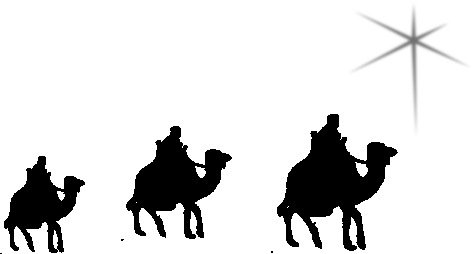
\includegraphics[height=2.8cm]{images/3kings_camels_star.pdf}
\end{center}

Vous allez discrètement rejetter Jésus-Christ si vous vous méprenez sur qui Il est. Jésus était et Il est Dieu incarné, le Dieu homme parfait et sans péché qui est venu pour réconcilier l'homme pécheur et impur à un Dieu saint et sans péché. Nous honorons Jésus seulement quand nous comprenons pleinement qui Il est, et combien nous avons besoin de Lui.
\nowidow[4]

\dvquote{%
Car vous connaissez la grâce de notre Seigneur Jésus-Christ qui pour vous s’est fait pauvre de riche qu’il était, afin que par sa pauvreté vous soyez enrichis.}{\ibibleverse{IICo}(8:9)}

\ornrule

\dvquote{%
Le salut ne se trouve en aucun autre; car il n’y a sous le ciel aucun autre nom donné parmi les hommes, par lequel nous devions être sauvés.}{%
\ibibleverse{Ac}(4:12)} 



